% Author Name: José Areia 
% Author Contact: jose.apareia@gmail.com
% Version: 2.2.9 - 2025-06-23
% Public Repository: https://github.com/joseareia/ipleiria-thesis
% Wiki/Getting Help: https://github.com/joseareia/ipleiria-thesis/wiki

%%% Document Options %%%
\documentclass[
    language=english,
    school=estg,
    docstage=final,
    media=screen,
    bookprint=false,
    linkcolor=blue!45!black,
    chapterstyle=classic,
    coverstyle=classic,
    aiack=false
]{IPLeiriaThesis} % Refer to the Wiki for a list of available options.

%%% Document Version %%%
\DocumentVersion{1.0.0} % Required only if the 'docstage' is set to 'working'.

%%% Document Metadata %%%
% First Author (Mandatory)
\FirstAuthor{Hyungmin Lim}
\FirstAuthorNumber{2022142207}

% Second Author (Optional)
% \SecondAuthor{Jane Smith}
% \SecondAuthorNumber{2230456}

% Third Author (Optional)
% \ThirdAuthor{July Smith}
% \ThirdAuthorNumber{2230457}

% Supervisor (Mandatory)
\Supervisor{Chaeyeon Park}
\SupervisorMail{chae-yeun@yonsei.ac.kr}
% Please provide: [Current Title, Affiliation]
\SupervisorTitle{Assistant Professor, Yonsei University} 

% Co-Supervisor (Optional)
% \CoSupervisor{Steve Smith}
% \CoSupervisorMail{steve.smith@ipleiria.pt}
% \CoSupervisorTitle{Associate Professor, Polytechnic of Leiria}

% Second Co-Supervisor (Optional)
% \SecCoSupervisor{Shak Smith}
% \SecCoSupervisorMail{shak.smith@ipleiria.pt}
% \SecCoSupervisorTitle{Associate Researcher, Computer Science \& Communication Research Centre}

% Title (Mandatory)
\Title{IBM Quantum Learning Course Guide}

% Subtitle (Mandatory)
\Subtitle{From Quantum mechanics to \\ Quantum diagonalization algorithms}

% University (Mandatory)
\University{Yonsei University}

% School (Mandatory)
\School{School of Engineering}

% Department (Mandatory)
\Department{Department of Electrical Engineering}

% Degree (Mandatory)
\Degree{Bachelor in Science}

% Course (Optional)
% \Course{Offensive \& Defensive Cybersecurity}

% Thesis Theme (Mandatory)
\ThesisType{Club Activity/QIYA/IBM Learning Course}

% Local & Date (Mandatory)
\Date{South Korea, \DTMmonthname{\month} \number\year}

% Academic Year 
\AcademicYear{2024/25}

%%% Loading of Glossary and Acronyms %%%
\makeglossaries
\loadglsentries{Matter/05-Glossary}
\loadglsentries[\acronymtype]{Matter/06-Acronyms}

\begin{document}

%%% Front Matter %%%
\ifthenelse{\equal{\CoverOption}{classic}}{
    \newcommand\BackgroundPicCover{%
    \put(0,0){%
    \parbox[b][\paperheight]{\paperwidth}{%
    \vfill
    \centering
    
\includegraphics[width=\paperwidth,height=\paperheight,keepaspectratio]{Figures/Theme/Cover-Blue.pdf}%
    \vfill
    }}}
}{
    \newcommand\BackgroundPicCover{%
    \put(0,0){%
    \parbox[b][\paperheight]{\paperwidth}{%
    \vfill
    \centering
    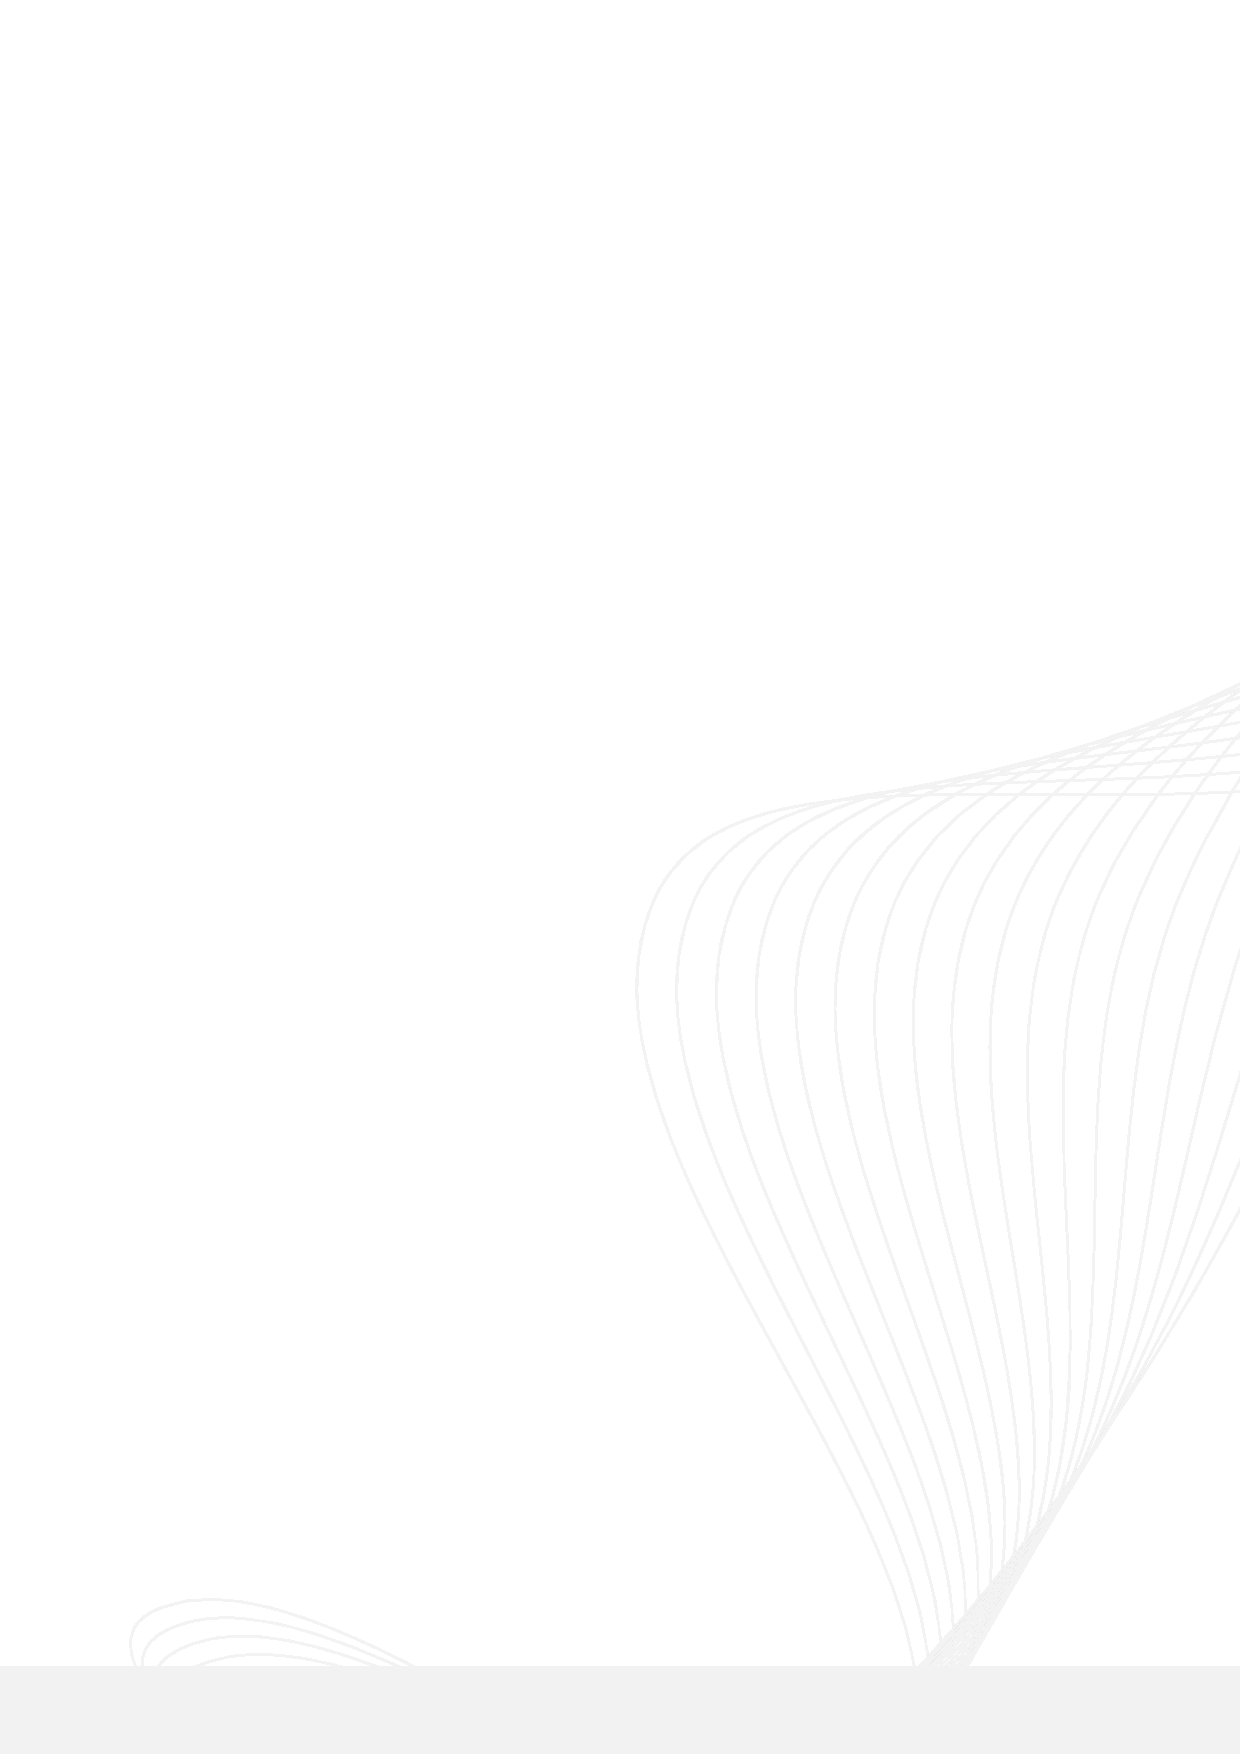
\includegraphics[width=\paperwidth,height=\paperheight,keepaspectratio]{Figures/Theme/Front-Page-BG.pdf}%
    \vfill
    }}}
}

\AddToShipoutPictureBG*{\BackgroundPicCover}

\newgeometry{margin=1.98cm, top=2.15cm, bottom=1.47cm}
\begin{titlepage}
    \IBMfont
    \ifthenelse{\equal{\CoverOption}{classic}}{\color{white}}{\color{frontpagedark}}
    \vspace*{\baselineskip}

    \ifthenelse{\equal{\CoverOption}{classic}}{

        \ifthenelse{\equal{\SchoolOption}{estg}}{
            \begin{figure}
                
\includegraphics[width=0.32\linewidth]{Figures/Theme/Logotypes/yslogo_full_white.pdf}
            \end{figure}
        }{}
        
        \ifthenelse{\equal{\SchoolOption}{esad}}{
            \begin{figure}
                
\includegraphics[width=0.485\linewidth]{Figures/Theme/Logotypes/IPLeiria-ESAD-Logo-W.pdf}
            \end{figure}
        }{}
        
        \ifthenelse{\equal{\SchoolOption}{esslei}}{
            \begin{figure}
                
\includegraphics[width=0.485\linewidth]{Figures/Theme/Logotypes/IPLeiria-ESSLEI-Logo-W.pdf}
            \end{figure}
        }{}
        
        \ifthenelse{\equal{\SchoolOption}{estm}}{
            \begin{figure}
                
\includegraphics[width=0.485\linewidth]{Figures/Theme/Logotypes/IPLeiria-ESTM-Logo-W.pdf}
            \end{figure}
        }{}
        
        \ifthenelse{\equal{\SchoolOption}{esecs}}{
            \begin{figure}
                
\includegraphics[width=0.485\linewidth]{Figures/Theme/Logotypes/IPLeiria-ESECS-Logo-W.pdf}
            \end{figure}
        }{}
    } {
        \ifthenelse{\equal{\SchoolOption}{estg}}{
            \begin{figure}
                
\includegraphics[width=0.485\linewidth]{Figures/Theme/Logotypes/IPLeiria-ESTG-Logo-B.pdf}
                % 
\includegraphics[width=0.4\linewidth]{Figures/Theme/Logotypes/IPLeiria-ESTG-Logo-Old.png}
            \end{figure}
        }{}
        
        \ifthenelse{\equal{\SchoolOption}{esad}}{
            \begin{figure}
                
\includegraphics[width=0.485\linewidth]{Figures/Theme/Logotypes/IPLeiria-ESAD-Logo-B.pdf}
            \end{figure}
        }{}
        
        \ifthenelse{\equal{\SchoolOption}{esslei}}{
            \begin{figure}
                
\includegraphics[width=0.485\linewidth]{Figures/Theme/Logotypes/IPLeiria-ESSLEI-Logo-B.pdf}
            \end{figure}
        }{}
        
        \ifthenelse{\equal{\SchoolOption}{estm}}{
            \begin{figure}
                
\includegraphics[width=0.485\linewidth]{Figures/Theme/Logotypes/IPLeiria-ESTM-Logo-B.pdf}
            \end{figure}
        }{}
        
        \ifthenelse{\equal{\SchoolOption}{esecs}}{
            \begin{figure}
                
\includegraphics[width=0.485\linewidth]{Figures/Theme/Logotypes/IPLeiria-ESECS-Logo-B.pdf}
            \end{figure}
        }{}
    }

    \vspace{5.5\baselineskip}

    % Title.
	\noindent
    \makebox[\textwidth][l]{%
        \parbox{\dimexpr\textwidth-4cm\relax}{
            \setstretch{1.03}
            \raggedright\bfseries\fontsize{22}{26}\selectfont\GetTitle
        }
    }

    \vspace{0.8\baselineskip}

    % Subtitle.
    \noindent
    \makebox[\textwidth][l]{%
        \parbox{\dimexpr\textwidth-7cm\relax}{
            \setstretch{1.03}
            \raggedright\fontsize{14}{19}\selectfont\GetSubtitle
        }
    }

    \vspace{35pt}  

    % Author.
    {\noindent\bfseries\fontsize{14}{19}\selectfont\GetFirstAuthor}

    \ifdefined\GetSecondAuthor
        \vspace{8pt}
        {\noindent\bfseries\fontsize{14}{19}\selectfont\GetSecondAuthor}
	\fi

    \ifdefined\GetThirdAuthor
        \vspace{8pt}
        {\noindent\bfseries\fontsize{14}{19}\selectfont\GetThirdAuthor}
	\fi
 
	\vfill

    % School.
	{\noindent\fontsize{10}{12}\selectfont\GetSchool}
	
    % Department.
	{\noindent\fontsize{10}{12}\selectfont\GetDepartment}

    % Degree.
	{\noindent\fontsize{10}{12}\selectfont\GetDegree}

    % Course.
    \ifdefined\GetCourse
        {\noindent\fontsize{10}{12}\selectfont\GetCourse}
	\fi

    \ifthenelse{\equal{\DocStageOption}{working}}{
        \vspace{62pt}
        {\noindent\fontsize{10}{12}\selectfont\overwritecolor{yellow}{\GetDocumentVersion \\ \textit{\today}}} 
        \vspace{62pt}
    }{
        \vspace{125pt}
    }

    % Local & Date.
	{\noindent\fontsize{10}{12}\selectfont\GetDate}

    \vspace{68pt}
\end{titlepage}
\restoregeometry
\MediaOptionLogic
\newcommand\BackgroundPicFrontPage{%
    \put(0,0){%
    \parbox[b][\paperheight]{\paperwidth}{%
    \vfill
    \centering
    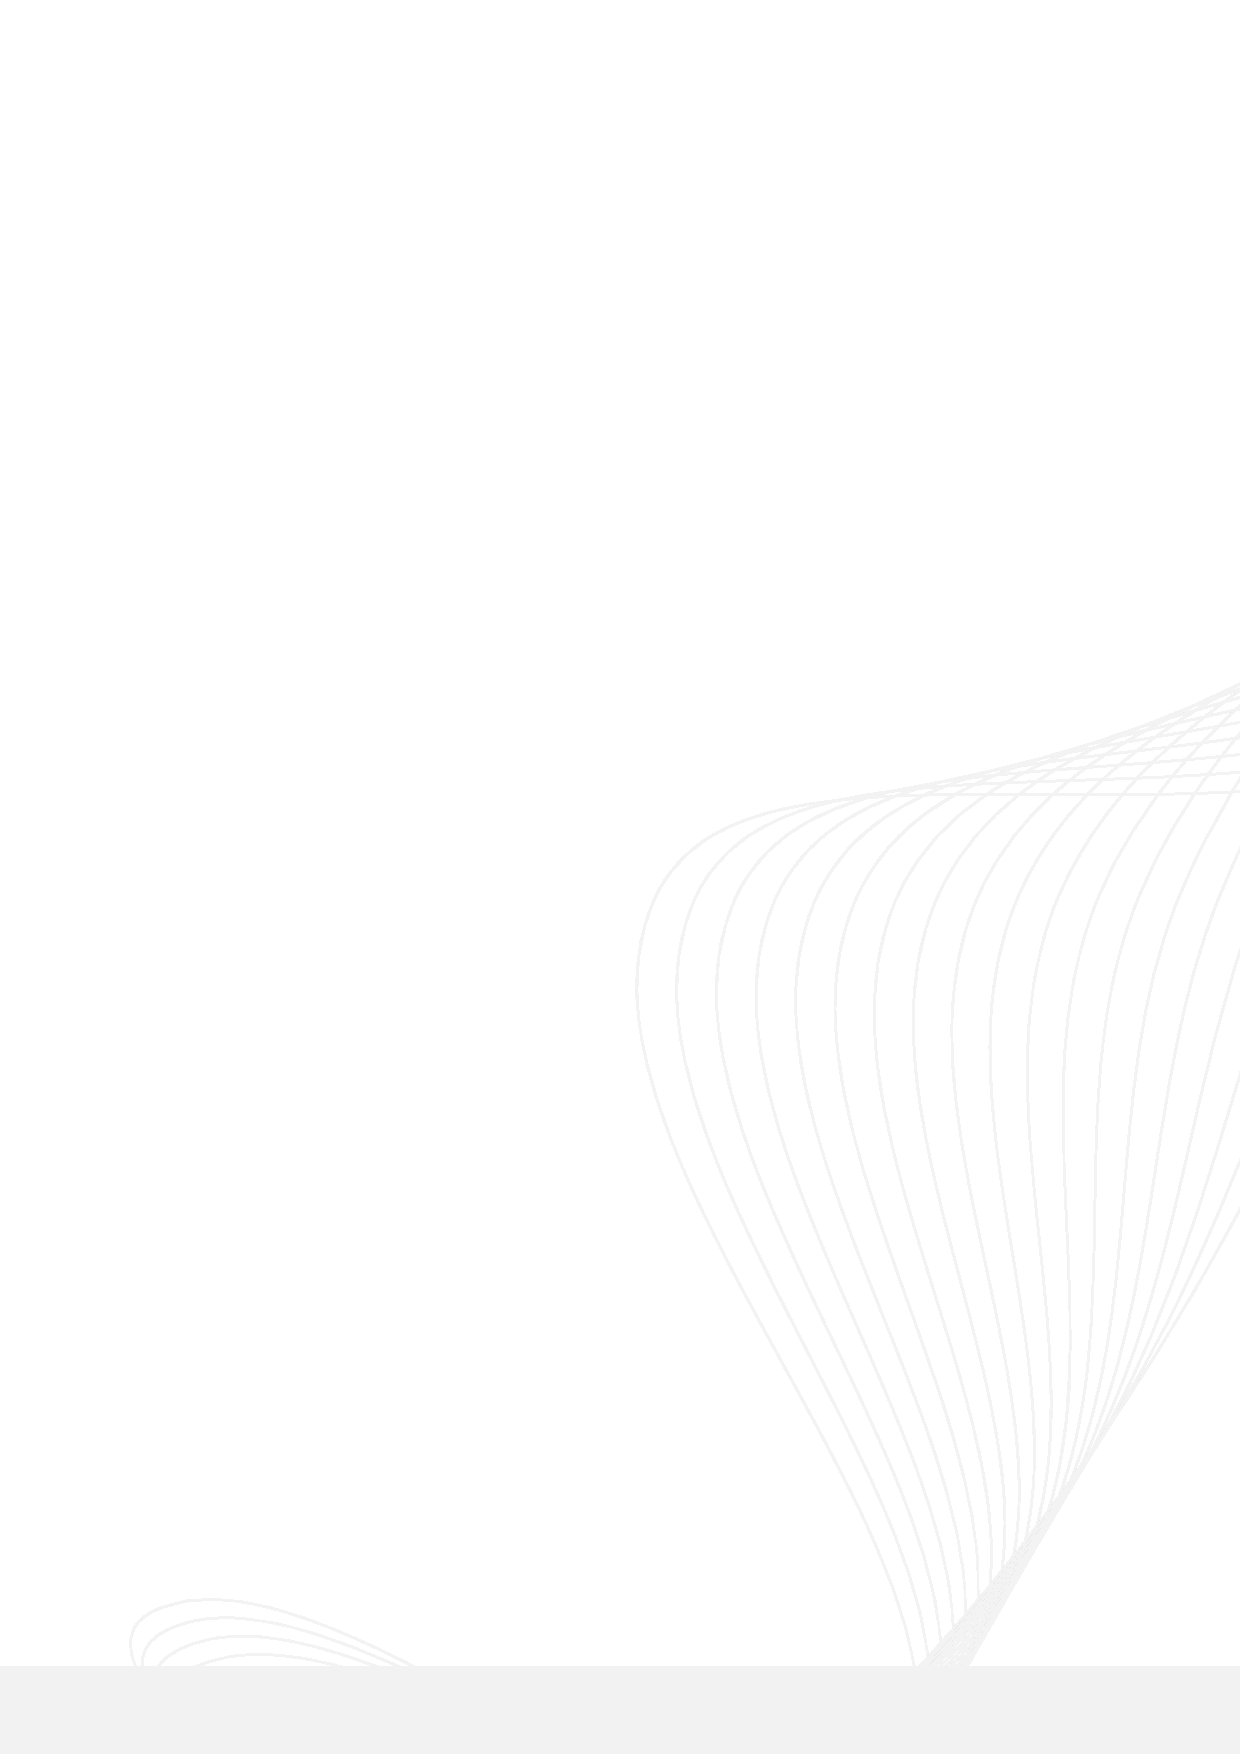
\includegraphics[width=\paperwidth,height=\paperheight,keepaspectratio]{Figures/Theme/Front-Page-BG.pdf}%
    \vfill
}}}
\AddToShipoutPictureBG*{\BackgroundPicFrontPage}

\newgeometry{margin=1.98cm, top=2.15cm, bottom=1.47cm}
\begin{titlepage}
    \IBMfont
    \color{frontpagedark}
    \vspace*{\baselineskip}

    \ifthenelse{\equal{\SchoolOption}{estg}}{
        \begin{figure}
            
\includegraphics[width=0.32\linewidth]{Figures/Theme/Logotypes/yslogo_full_black.pdf}
            % 
\includegraphics[width=0.4\linewidth]{Figures/Theme/Logotypes/IPLeiria-ESTG-Logo-Old.png}
        \end{figure}
    }
    
    \ifthenelse{\equal{\SchoolOption}{esad}}{
        \begin{figure}
            
\includegraphics[width=0.485\linewidth]{Figures/Theme/Logotypes/IPLeiria-ESAD-Logo-B.pdf}
        \end{figure}
    }
    
    \ifthenelse{\equal{\SchoolOption}{esslei}}{
        \begin{figure}
            
\includegraphics[width=0.485\linewidth]{Figures/Theme/Logotypes/IPLeiria-ESSLEI-Logo-B.pdf}
        \end{figure}
    }
    
    \ifthenelse{\equal{\SchoolOption}{estm}}{
        \begin{figure}
            
\includegraphics[width=0.485\linewidth]{Figures/Theme/Logotypes/IPLeiria-ESTM-Logo-B.pdf}
        \end{figure}
    }
    
    \ifthenelse{\equal{\SchoolOption}{esecs}}{
        \begin{figure}
            
\includegraphics[width=0.485\linewidth]{Figures/Theme/Logotypes/IPLeiria-ESECS-Logo-B.pdf}
        \end{figure}
    }

    \vspace{3.5\baselineskip}

    % Title.
	\noindent
    \makebox[\textwidth][l]{%
        \parbox{\dimexpr\textwidth-2.5cm\relax}{
            \setstretch{1.03}
            \raggedright\bfseries\fontsize{22}{26}\selectfont\GetTitle
        }
    }

    \vspace{0.8\baselineskip}

    % Subtitle.
    \noindent
    \makebox[\textwidth][l]{%
        \parbox{\dimexpr\textwidth-7cm\relax}{
            \setstretch{1.03}
            \raggedright\fontsize{14}{19}\selectfont\GetSubtitle
        }
    }

    \vspace{35pt}

    % Author.
    {\noindent\bfseries\fontsize{14}{19}\selectfont\GetFirstAuthor}
    
    {\noindent\itshape\fontsize{10}{10}\selectfont Student No. \GetFirstAuthorNumber}

    \ifdefined\GetSecondAuthor
        \vspace{8pt}
        {\noindent\bfseries\fontsize{14}{19}\selectfont\GetSecondAuthor}
	\fi

    \ifdefined\GetThirdAuthor
        \vspace{8pt}
        {\noindent\bfseries\fontsize{14}{19}\selectfont\GetThirdAuthor}
	\fi

    \vspace{58pt}    

    {
    \noindent
    \latofont
    \fontsize{10}{12}\selectfont
    \renewcommand{\arraystretch}{0.1}
    \hspace*{-2.5pt}\begin{tabular}{@{}r@{\hspace{5pt}}>{\raggedright\arraybackslash}m{6cm}@{}}
        \textbf{Supervisor:} & \GetSupervisor \\ [-.7ex]
        & \setstretch{0.9}{\fontsize{8}{10}\selectfont\itshape \GetSupervisorTitle} \\ [2ex]
        
        \ifdefined\GetCoSupervisor
            \textbf{Co-supervisor:} & \GetCoSupervisor \\ [-.7ex]
            & \setstretch{0.9}{\fontsize{8}{10}\selectfont\itshape \GetCoSupervisorTitle} \\ [.5ex]
        \fi

        \ifdefined\GetSecCoSupervisor        
            & \GetSecCoSupervisor \\ [-.7ex]
            & \setstretch{0.9}{\fontsize{8}{10}\selectfont\itshape \GetSecCoSupervisorTitle} \\
        \fi
    \end{tabular}
    }
    
    \vfill
	
    % School.
	{\noindent\fontsize{10}{12}\selectfont\GetSchool}
	
    % Department.
	{\noindent\fontsize{10}{12}\selectfont\GetDepartment}

    % Degree.
	{\noindent\fontsize{10}{12}\selectfont\GetDegree}

    % Course.
    \ifdefined\GetCourse
        {\noindent\fontsize{10}{12}\selectfont\GetCourse}
	\fi

    \vspace{45pt}

    % Thesis option.
	{\noindent\fontsize{10}{12}\itshape\selectfont\GetThesisType}

    \vspace{45pt}

    % Local and date.
	{\noindent\fontsize{10}{12}\selectfont\GetDate}

    \vspace{68pt}
\end{titlepage}
\restoregeometry
\MediaOptionLogic

%%% Copyright Statement %%%
\pagenumbering{gobble} % Prevent page numbering.

\vspace*{\fill}

% \ifthenelse{\equal{\LanguageOption}{portuguese}}{%
%     \noindent \textbf{\GetTitle}
    
%     \noindent Copyright \textcopyright~\the\year{} - \GetFirstAuthor, \GetSchool.
    
%     \vspace{.575em}
    
%     \noindent A presente dissertação é um trabalho original, elaborado exclusivamente para este fim, tendo sido devidamente citados todos os autores cujos estudos contribuíram para a sua elaboração. É permitida a sua reprodução parcial com indicação do autor e referência ao grau, ano letivo, instituição---\textit{Politécnico de Leiria}---e data da defesa pública.

%     \vspace{1.395em}
    
%     \noindent\psvectorian[scale=.25,opacity=.80]{2}
    
%     \vspace{.935em}

%     \noindent O presente trabalho beneficiou da utilização do modelo \textit{IPLeiria-Thesis}.
% }{%
% }


\noindent \textbf{\GetTitle}

\noindent Copyright \textcopyright~\the\year{} - \GetFirstAuthor, \GetSchool.

\vspace{.575em}

% \noindent This dissertation is original work, written solely for this purpose, and all the authors whose studies and publications contributed to it have been duly cited. Partial reproduction is allowed with acknowledgment of the author and reference to the degree, academic year, institution---\textit{Polytechnic University of Leiria}---and public defense date.

\noindent This dissertation is original work, written solely for guiding QIYA students, and all the authors whose studies and publications contributed to it have been duly cited. Partial reproduction is allowed with acknowledgment of the author and reference to the degree, academic year, institution---\textit{Yonsei University}---and public defense date.

\vspace{1.395em}

% Pst-vectorian is NOT available since 2022 due to no maintanance
% \noindent\psvectorian[scale=.25,opacity=.80]{2}

\begin{center}
\pgfornament[width=4cm,color=black!60]{88}
\end{center}


\vspace{.935em}

\noindent Preparation of this work was facilitated by the use of the \href{https://github.com/joseareia/ipleiria-thesis}{\textit{IPLeiria-Thesis}} template.

\vspace*{\fill}
\MediaOptionLogic

%%% Roman Numeration %%%
\pagenumbering{roman}

%%% Acknowledgements %%%
\ifthenelse{\equal{\LanguageOption}{portuguese}}{%
    \chapter*{Agradecimentos}
}{%
    \chapter*{Acknowledgements}
}

% \guideinfo{In the \textit{Acknowledgment} section, express your gratitude to those who helped and supported your work. Start by thanking your advisors, mentors, or supervisors who provided guidance and expertise. Mention any colleagues, classmates, or team members who contributed to discussions or offered assistance. You can also acknowledge specific organisations, institutions, or funding sources that supported your research or work. Lastly, include any personal acknowledgments for family or friends who offered encouragement and moral support during the project. Keep this section sincere, concise, and professional.}

I would like to express my deepest gratitude to Professor Chaeyeon Park, whose guidance and encouragement were invaluable throughout the preparation of this project. Her insights and unwavering support made this work possible.

I am also sincerely thankful to Junseok Jung, a graduate student whose thoughtful advice and expertise provided me with both technical direction and motivation during the development process.

Special thanks go to my close friends and collaborators, Seokwon Choi and Jungbin Ho, for their active participation in discussions and their companionship throughout the IBM Quantum Learning Course. Their presence made this journey both intellectually rewarding and personally meaningful.

Finally, I would like to acknowledge the organizers and contributors of the IBM Quantum Learning Course, whose efforts in designing and delivering the program laid the foundation for this project. Their dedication to advancing quantum education was a true inspiration.


\MediaOptionLogicBlank

%%% Abstract %%%
\thispagestyle{plain}
\pdfbookmark[1]{Abstract}{abstract}
\chapter*{Abstract}
% \guideinfo{In the \textit{Abstract} section, provide a concise summary of your project, highlighting the key points. Begin with a brief statement of the problem or objective, followed by a description of your approach or methodology. Summarise the main results or findings, emphasising their significance or implications. Conclude with a sentence or two on the overall contribution or impact of your work. Keep the abstract clear and focused, ideally within 150-250 words, to give readers a quick understanding of your research and its importance.}

This guide is intended for those who are beginning their study of quantum information and its implementation using Qiskit. It is originally based on the \href{https://quantum.cloud.ibm.com/learning/en}{IBM Learning Course}. The document primarily covers seven modules from the course: Quantum Mechanics, Computer Science, Basics of Quantum Information, Fundamentals of Quantum Algorithms, General Formulation of Quantum Information, Foundations of Quantum Error Correction, Quantum Computing in Practice, and Quantum Chemistry with VQE and Quantum Diagonalization Algorithms.
Each topic is grounded in deep mathematical and technical foundations, but the IBM course is designed to be accessible to general audiences. This guide aims to elaborate on the content of these modules and provide detailed explanations and answers to the accompanying discussion problems.

\keywordsen{Quantum Information Basics, Quantum Algorithm Basics.}

\MediaOptionLogicBlank

%%% AI Acknowledgement %%%
% \ifthenelse{\equal{\AiAckOption}{true}}{%
    \ifthenelse{\equal{\LanguageOption}{portuguese}}{%
        \chapter*{Declaração sobre o Uso de Inteligência Artificial}

        \guideinfo{É uma boa prática académica indicar brevemente como, porquê e quando a IA foi utilizada. Explicar as ações tomadas e as razões que lhes estão subjacentes promove a reflexão crítica, aprofunda a compreensão do papel da IA na aprendizagem e ajuda a avaliar o seu impacto na qualidade e integridade do trabalho. Esta página pode ser removida definindo a opção \texttt{aiack} como \texttt{false} nas opções da classe do documento.}
    
        \vspace{2em}
        
        \exampleinfo{%
        Reconheço a utilização do ChatGPT (\url{https://chatgpt.com}) para aperfeiçoar o tom académico e melhorar a precisão linguística deste trabalho, incluindo aspectos de gramática, pontuação e vocabulário.
        
        \vspace{1em}
        
        \noindent\textbf{Descrição da Utilização}
        
        \prompt[1]{Num parágrafo, descreva simplesmente o que é o LaTeX.}
        
        \aioutput[1]{O LaTeX é um sistema de composição de alta qualidade, normalmente utilizado para produzir documentos científicos e matemáticos, devido ao seu poderoso manuseamento de fórmulas e bibliografias. Ao contrário dos processadores de texto, utiliza ficheiros de texto simples com etiquetas de marcação para definir a estrutura e a formatação de um documento, permitindo um controlo preciso da disposição e do aspeto. É especialmente popular no meio académico e na investigação para a criação de teses, artigos de revistas e apresentações.}
        }
    }{%
        \chapter*{AI Acknowledgement}

        \guideinfo{It is good academic practice to briefly state how, why, and when AI was used. Explaining both the actions taken and the reasons behind them encourages critical reflection, deepens understanding of AI's role in learning, and supports the evaluation of its impact on your work’s quality and integrity. This page can be removed by setting the option \texttt{aiack} to \texttt{false} in the document class options.}

        \vspace{2em}
        
        \exampleinfo{%
        I acknowledge the use of ChatGPT (\url{https://chatgpt.com}) to refine the academic tone and improve the linguistic accuracy of this work, including aspects of grammar, punctuation, and vocabulary.
        
        \vspace{1em}
        
        \noindent\textbf{Description of Use}
        
        \prompt[1]{In a paragraph, simply describe what LaTeX is.}
        
        \aioutput[1]{LaTeX is a high-quality typesetting system commonly used for producing scientific and mathematical documents due to its powerful handling of formulas and bibliographies. Unlike word processors, it uses plain text files with markup tags to define the structure and formatting of a document, allowing precise control over layout and appearance. It is especially popular in academia and research for creating theses, journal articles, and presentations.}
        }
    }
    
    \MediaOptionLogicBlank   
}{}

%%% Table of Contents, List of Figures and List of Tables %%%
\bookmarktocentry\tableofcontents
\listoffigures
\listoftables

%%% Print: Glossary and Acronyms %%%
% \glossarytoc\printnormalglossary
% \acronymtoc\printacronymglossary

%%% Arabic Numeration %%%
\pagenumbering{arabic}

%%% Chapters (**Insert Yours Here**) %%%
\chapter[Qiskit in Classrooms: Quantum Mechanics]{Qiskit in Classrooms: Quantum Mechanics}
\label{cp:introduction}

\parindent0pt

\textit{Author: Hyungmin Lim}

\textit{Current Version: 0.0.1}

\textit{License: \LaTeX~Project Public License v1.3c}

\textit{Official Repository: \href{https://github.com/joseareia/ipleiria-thesis}{GitHub Repository}}

\vspace{.935em}

Welcome to the \textcolor{maincolor}{\textit{IBM Quantum Learning Course Guide}}! 

\section{Superposition with Qiskit}

In this section, we will find out the one of the most important quantum phenomenon-superposition. Through 


\section{Stern-Gelach measurements with Qiskit}

\subsection{Introduction}
\subsection{Classical coin}
\subsection{Quantum coin}
\subsection{The quantum revealed: an experiment in three dimensions}
\subsection{The quantum phase}
\subsection{Bloch sphere representation}
\subsubsection{Blochsphere examples}
Hello my freinds


\section{Exploring uncertainty with Qiskit}


\section{Bell's inequality with Qiskit}
% \chapter[Comprehensive User Guide: Instructions for Using the Template]{Comprehensive User Guide Instructions for Using the Template}
\label{cp:user-guide}

If you plan to use this template, please read this chapter carefully. It provides all the information you need to effectively use the template, including the mandatory modifications (\textit{e.g.}, title, subtitle, author information) and other configurations that, while not highly recommended, are optional. The template comprises various directories and files, including a total of seven distinct directories and dozens of files. Among these, the most important are \texttt{IPLeiriaMain.tex} and \texttt{IPLeiriaThesis.cls}. Below, \autoref{tab:file-structure} presents the different directories available, along with their descriptions and a check-mark indicating whether you need to access the directory to make changes. Of course, the check mark indicates that you can make changes to the content, while a hyphen signifies that you should not modify it.

\begin{table}[!htpb]
    \setlength{\extrarowheight}{2pt}
    \caption[Directory structure and file organisation]{Overview of the directory structure in this template.}
    \label{tab:file-structure}
    \begin{tabularx}{\textwidth}{lcX}
        \toprule
        \\[-1.5\normalbaselineskip]
        \textbf{Directory} & \textbf{Modifiable} & \textbf{Description} \\ [0em]
        \midrule
        \textit{Bibliography} & $\checkmark$ & This folder contains the bibliography file used to manage references throughout the document. \\
        \textit{Chapters} & $\checkmark$ & Individual chapters of the thesis are organised in this directory, making it easy to work on sections separately. \\
        \textit{Code} & $\checkmark$ & Code examples and relevant scripts are stored here, supporting the content of the thesis. \\
        \textit{Configurations} & - & All configuration files required for the template, such as layout and style settings, are placed in this directory. \\
        \textit{Figures} & $\checkmark$ & All figures and images referenced within the document are stored in this folder for easy access and management. \\
        \textit{Matter} & - & The front matter of the document, including the cover page, copyright statement, and glossary, is assembled in this directory. \\
        \textit{Metadata} & $\checkmark$ & This folder holds the metadata file, where key document details such as the author, title, and supervisor can be customised. \\
        \bottomrule
    \end{tabularx}
\end{table}

It is crucial to note that the files are organised according to a specific naming convention, which must be \textbf{respected} and \textbf{maintained}. The naming convention consists of an ascending two-digit numeric value, followed by a hyphen, and then the file name in capital letters. The name should always aim to be a single word. If more than one word is necessary, they should be separated by a hyphen and capitalised.

\begin{block}[note]
While \autoref{tab:file-structure} indicates that the \textit{Matter} directory is not modifiable, two files within that directory should be altered when necessary: \texttt{04-Glossary.tex} and \texttt{05-Acronyms.tex}. Although the names are fairly self-explanatory, these files should contain the glossary and acronyms entries, respectively.
\end{block}

The two files mentioned earlier, \texttt{IPLeiriaMain.tex} and \texttt{IPLeiriaThesis.cls}, should be used with caution. The main file, as the name suggests, is the master file where you will add the necessary chapters to be included in your work. The class file, on the other hand, requires even more caution, and it is not recommended to alter it.

\section{Template and Class Options}
\label{sec:class-options}
The first thing you need to do is specify the options within the \texttt{IPLeiriaMain.tex} file. How do you do that? It's simple. On the very first line, you will find a \texttt{documentclass} command that loads the custom class for this template. In this call, you can pass the options you need. The available options, presented in a key-argument style, are listed in \autoref{tab:template-options}.

{
\setlength{\extrarowheight}{-1.75pt}
\begin{xltabular}{\textwidth}{lX}
\caption{Class options supported by the template.}
\label{tab:template-options} \\
%
\toprule 
\multicolumn{1}{l}{\textbf{Options}} & \multicolumn{1}{l}{\textbf{Description}} \\ 
\midrule
\endfirsthead
%
\multicolumn{2}{c}%
{{\textit{\bfseries Table \thetable\ continued from previous page.}}} \\
%
\toprule 
\multicolumn{1}{l}{\textbf{Options}} & \multicolumn{1}{l}{\textbf{Description}} \\ 
\midrule
\endhead
%
\bottomrule
\addlinespace[1mm]
\multicolumn{2}{r}%
{{\textit{Continued on the next page.}}} \\
\endfoot
\bottomrule
\endlastfoot

\textbf{school=OPT} & \textbf{Choosing a school and its corresponding logo.} \\
\multirow[t]{2}{*}{\footnotesize{\textit{estg, esecs, esslei, esad, estm}}} & \footnotesize{\textit{$\Rightarrow$ Default: school=estg}} \\
& \footnotesize{\textit{This option only modifies the school name and the corresponding logo, which will be displayed on the cover and front page.}} \\[1.70em]

\textbf{language=OPT} & \textbf{Language preference selection.} \\
\footnotesize{\textit{portuguese, english}} & \footnotesize{\textit{$\Rightarrow$ Default: language=english}} \\[0.85em]
        
\textbf{chapterstyle=OPT} & \textbf{Selection of a cover design style.} \\
\multirow[t]{2}{*}{\footnotesize{\textit{classic, modern, fancy}}} & \footnotesize{\textit{$\Rightarrow$ Default: chapterstyle=classic}} \\
& \footnotesize{\textit{This option modifies the appearance of the chapter, including its title and numbering style. Explore the available styles and apply the one you prefer.}} \\[1.70em]

\textbf{coverstyle=OPT} & \textbf{Choosing a style for the chapter.} \\
\multirow[t]{3}{*}{\footnotesize{\textit{classic, bw}}} & \footnotesize{\textit{$\Rightarrow$ Default: coverstyle=classic}} \\
& \footnotesize{\textit{classic $\rightarrow$ Put the cover on in the original red.}} \\
& \footnotesize{\textit{bw $\rightarrow$ Make the cover black and white.}} \\

\textbf{docstage=OPT} & \textbf{Choosing a stage for you document.} \\
\multirow[t]{3}{*}{\footnotesize{\textit{final, working}}} & \footnotesize{\textit{$\Rightarrow$ Default: docstage=final}} \\
& \footnotesize{\textit{final $\rightarrow$ Assumes this is the final version of the document.}} \\
& \footnotesize{\textit{working $\rightarrow$ It assumes the document is a work in progress.}} \\[.3em]

\textbf{media=OPT} & \textbf{Project media type.} \\
\multirow[t]{3}{*}{\footnotesize{\textit{paper, screen}}} & \footnotesize{\textit{$\Rightarrow$ Default: media=paper}} \\
& \footnotesize{\textit{paper $\rightarrow$ Blank pages will appear between sections.}} \\
& \footnotesize{\textit{screen $\rightarrow$ Blank pages will not appear between sections.}} \\[.3em]

\textbf{linkcolor=OPT} & \textbf{Main theme color.} \\
\multirow[t]{2}{*}{\footnotesize{\textit{color}}} & \footnotesize{\textit{$\Rightarrow$ Default: linkcolor=red!45!black}} \\
& \footnotesize{\textit{This option requires a valid color name. Refer to the xcolor manual (subsection 4.2) to select a valid color.}} \\[.3em]

\textbf{bookprint=OPT} & \textbf{For book printing.} \\
\multirow[t]{2}{*}{\footnotesize{\textit{true, false}}} & \footnotesize{\textit{$\Rightarrow$ Default: bookprint=false}} \\
& \footnotesize{\textit{This option adds a binding margin on odd-numbered pages to allow for printing, as it increases the left margin.}} \\[.3em]

\textbf{aiack=OPT} & \textbf{AI acknowledgement print.} \\
\multirow[t]{2}{*}{\footnotesize{\textit{true, false}}} & \footnotesize{\textit{$\Rightarrow$ Default: aiack=true}} \\
& \footnotesize{\textit{This option adds a section intended for the user to insert their acknowledgement of AI usage.}} \\
\end{xltabular}
}

After setting the desired options in the main class, you are all set to personalise the metadata. To learn how, simply refer to \autoref{sec:metadata}.

\section{Metadata Customisation}
\label{sec:metadata}
While options like language and school can be passed as arguments to the main class, other options, such as author and title, must be defined manually. Since this template supports a wide range of metadata options, a dedicated file is provided for this purpose. The file at \texttt{Metadata/Metadata.tex} lists metadata variables, with comments on whether they are mandatory. Comment out the variables to omit them. \autoref{tab:metadata} includes all metadata variables, their GET command, and if they are mandatory. The GET command automatically retrieves the information from the stored variable.

\begin{longtable}[c]{llc}
\caption{Metadata variables within the template.}
\label{tab:metadata} \\
\toprule
\textbf{Variable} & \textbf{Macro Commands} & \textbf{Mandatory} \\ \midrule
\endfirsthead
%
\multicolumn{3}{c}%
{{\textit{\bfseries Table \thetable\ continued from previous page.}}} \\
%
\toprule
\textbf{Variable} & \textbf{Macro Commands} & \textbf{Mandatory} \\ \midrule
\endhead
%
\bottomrule
%
\addlinespace[1mm]
\multicolumn{3}{r}%
{{\textit{Continued on the next page.}}} \\
\endfoot
%
\bottomrule
%
\endlastfoot
%
Title            & \verb|\GetTitle|         & $\checkmark$ \\
Subtitle         & \verb|\GetSubtitle|      & $\checkmark$ \\
University       & \verb|\GetUniversity|    & $\checkmark$ \\
School           & \verb|\GetSchool|        & $\checkmark$ \\
Department       & \verb|\GetDepartment|    & $\checkmark$ \\
Degree           & \verb|\GetDegree|        & $\checkmark$ \\
Course           & \verb|\GetCourse|        & -            \\
Local and date   & \verb|\GetDate|          & $\checkmark$  \\ 
Academic year    & \verb|\GetAcademicYear|  & $\checkmark$ \\ 

Thesis type (\scriptsize{\textit{Dissertation, Project or Internship}}) & \verb|\GetThesisType| & $\checkmark$ \\

First author name           & \verb|\GetFirstAuthor|        & $\checkmark$ \\
First author identification & \verb|\GetFirstAuthorNumber|  & $\checkmark$ \\ 

Second author name           & \verb|\GetSecondAuthor|          & - \\
Second author identification & \verb|\GetSecondAuthorNumber|    & - \\ 

Third author name           & \verb|\GetThirdAuthor|        & - \\
Third author identification & \verb|\GetThirdAuthorNumber|  & - \\ 

Supervisor name                  & \verb|\GetSupervisor|        & $\checkmark$ \\
Supervisor e-mail                & \verb|\GetSupervisorMail|    & $\checkmark$ \\
Supervisor title and affiliation & \verb|\GetSupervisorTitle|   & $\checkmark$ \\ 

Co-supervisor name                  & \verb|\GetCoSupervisor|       & - \\
Co-supervisor e-mail                & \verb|\GetCoSupervisorMail|   & - \\
Co-supervisor title and affiliation & \verb|\GetCoSupervisorTitle|  & - \\ 

Second co-supervisor name                   & \verb|\GetSecCoSupervisor|      & - \\
Second co-supervisor e-mail                 & \verb|\GetSecCoSupervisorMail|  & - \\
Second co-supervisor title and affiliation  & \verb|\GetSecCoSupervisorTitle| & - \\
\end{longtable}

If, by any chance, \textbf{you want to add more options}, please contact me by opening an issue in the official GitHub repository or via the email provided in this document.

\section{Custom Chapter Insertion}
As stated before, to use this template, you need to do three things: set the appropriate options in the document class (see \autoref{sec:class-options}), update the document metadata (see \autoref{sec:metadata}), and create and import your custom chapters. To create and import a custom chapter, follow these steps: \(i\) create a TeX file in the Chapters directory that follows the predefined naming convention and \(ii)\) include it in the main file using the command \verb|\include{CHAPTER}|. And voilà, your first chapter is ready!

\section{Custom Commands}
Within this template, some custom commands are also available for your use. For example, if you are writing your thesis and want to add a to-do note, you can easily insert a block with the option \verb|todo|, as follows: \verb|\begin{block}[todo]|. This will insert a to-do block with a style similar to Markdown. Other available options are: \verb|tip|, \verb|warning|, and \verb|note|. Below is a visual example for each one.

\vspace{.875em}
\begin{tcbraster}[
    raster columns=2, 
    raster equal height, 
    nobeforeafter, 
    raster column skip=1cm
]
\begin{block}[todo]
    This is a to-do block.
\end{block}
\begin{block}[tip]
    This is a tip block.
\end{block}
\end{tcbraster}

\begin{tcbraster}[
    raster columns=2, 
    raster equal height, 
    nobeforeafter, 
    raster column skip=1cm
]
\begin{block}[warning]
    This is a warning block.
\end{block}
\begin{block}[note]
    This is a note block.
\end{block}
\end{tcbraster}
\vspace{.875em}
% \chapter[Essential LaTeX Tutorial: Fundamentals and Key Concepts]{Essential LaTeX Tutorial Fundamentals and Key Concepts}
\label{cp:latex-tutorial}

This chapter introduces the \LaTeX~working environment and the essentials for producing your thesis. \LaTeX~(pronounced ``LAY-tek'' or ``LAH-tek'') is a tool for creating professional documents using plain text with formatting commands, unlike WYSIWYG editors like Microsoft Word. These files are processed by a TeX engine to generate a polished PDF, allowing you to focus on content while \LaTeX~handles the layout. While this chapter covers key features, it's worth learning \LaTeX~from the start. For a quick introduction, see Overleaf \href{https://www.overleaf.com/learn/latex/Learn_LaTeX_in_30_minutes}{Learn LaTeX} series for guidance.

\section{Citations}
\label{sec:citations}
We present two distinct approaches for citing entries in the bibliography. The first method involves in-text citations, executed using \verb|\citet{ENTRY}|, while the second method employs \verb|\citep{ENTRY}| for citations within a paragraph. Below is an example that demonstrates both usages. You can cite multiple works in the same citation environment using \verb|\citep{ENTRY1, ENTRY2, ...}|. For citing only the title, use \verb|\citetitle{ENTRY}|, and for the author, use \verb|\citeauthor{ENTRY}|.

\begin{block}[tip]
Proper citations are vital in academic writing and ensure credibility, transparency, and knowledge advancement. They are essential for responsible scholarship. Ensure accuracy and appropriateness.
\end{block}

\noindent\textbf{Example:} A novel signature scheme is introduced, along with an implementation of the Diffie-Hellman key distribution scheme that accomplishes a public key cryptosystem \citep{Elgamal1985}. According to \citet{Elgamal1985}, a new signature scheme that accomplishes a public key cryptosystem is introduced (...) This template was created by \citeauthor{IPLeiriaThesis}, with the title \citetitle{IPLeiriaThesis}.

\section{References}
Much like citations, it is advisable to employ references in your document for citing crucial elements such as chapters, sections, figures, or tables. To reference these elements, begin by creating a label. This label can be generated using \verb|\label{TEXT}|, and it should be positioned within the element you intend to refer to. Once the element is created, you can utilise \verb|\ref{LABEL}| to generate an in-text reference. \textbf{We strongly recommend using} \verb|\autoref{LABEL}|. This command automatically creates a custom link with color corresponding to the type of element being referred to. For instance, a chapter reference will appear like this: \autoref{cp:introduction}, rather than simply Chapter \ref{cp:introduction}. 

\begin{block}[tip]
Properly referencing elements within the document, such as \textbf{chapters, sections, figures, tables, or listings}, is crucial.
\end{block}

\section{Glossary and Acronyms}
The document includes both a glossary and an acronym list, accessible at the beginning of the document. You can create a new entry in either the \verb|Matter/02-Glossary| or \verb|Matter/03-Acronyms| sections, depending on the type of entry you intend to add. Once the entry is created, you can reference it using \verb|\gls{ENTRY}| for glossary entries. For acronym entries, there are two ways to reference them. The first method, \verb|\acrfull{ENTRY}|, should be used the first time the acronym appears in the text as it automatically provides the definition in-text. Subsequently, to refer to the acronym without repeating its meaning, use \verb|\acrshort{ENTRY}|.

\vspace{.875em}
\noindent\textbf{Example:} Utilising \Gls{latex} for \Gls{maths} is essential (...). It is advisable to seek both the \acrfull{gcd} and \acrfull{lcm} because (...). Subsequently, with the aid of \acrshort{gcd} and \acrshort{lcm}, we can (...).

\section{Figures}
In \LaTeX, integrating figures is a straightforward process. To insert them, you should utilise the environment \verb|\begin{figure}|. You can customise the \verb|width| parameter according to your requirements, but it is crucial to select a high-quality figure when inserting it into your documents. It is equally crucial to furnish a well-crafted caption. If necessary, consider including citations or references to indicate the figure's origin. The caption environment is denoted as \verb|\caption{TEXT}|. To generate a smaller caption for the Table of Figures, be sure to utilise the format \verb|\caption[SMALL_TEXT]{BIG_TEXT}|. By following the aforementioned tips, we can create a figure as demonstrated in \autoref{fig:figure-01}.

\begin{figure}[!htpb]
    \centering
    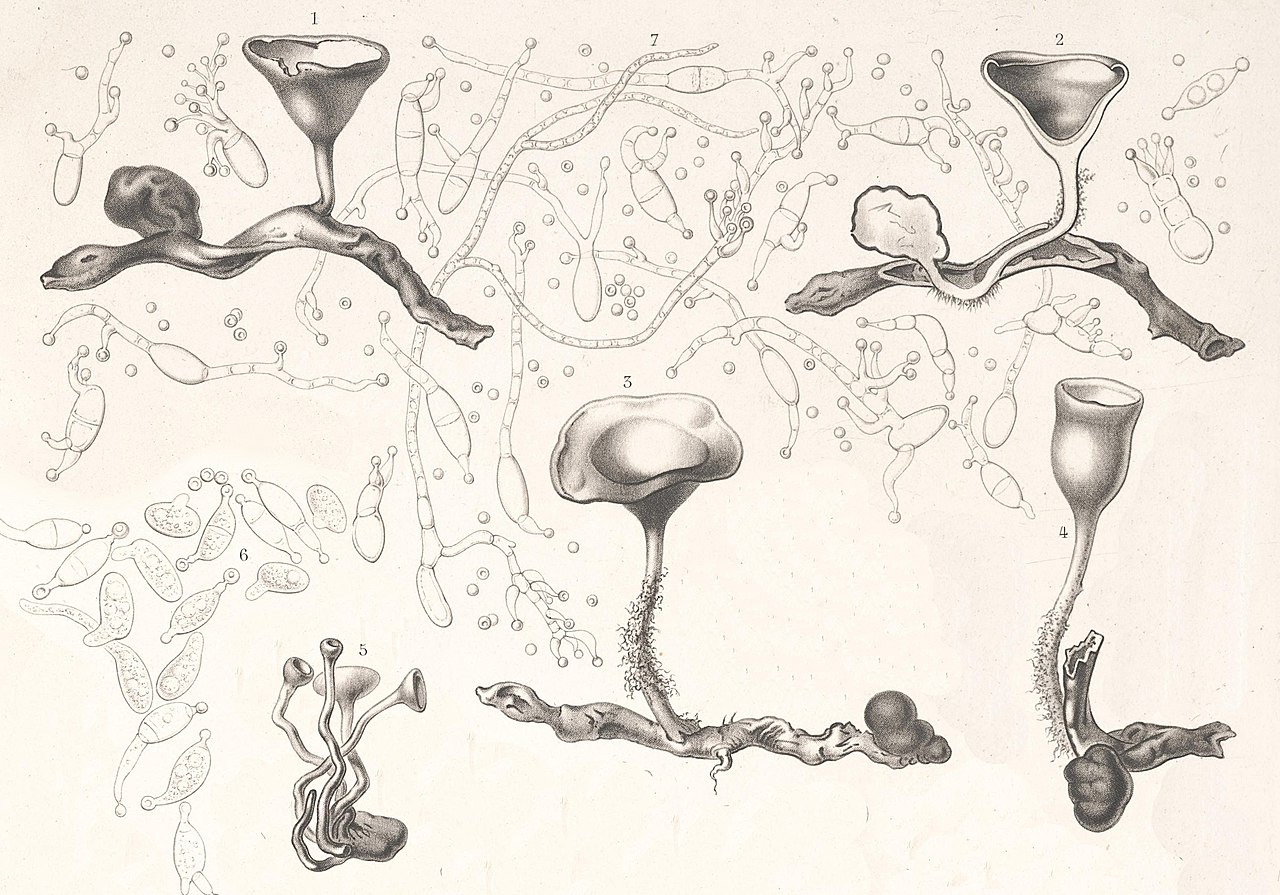
\includegraphics[width=\linewidth]{Figures/PezizaTuberosa.jpg}
    \caption[Illustration of the fungus Dumontinia tuberosa.]{Illustration of the fungus Dumontinia tuberosa by physician, mycologist, and illustrator Charles Tulasne (1816–1884) in the book Selecta Fungorum Carpologia (1861–65). (Name of the original work: Peziza tuberosa parasite on Anemone nemorosa).}
    \label{fig:figure-01}
\end{figure}

For comparison or for other reasons, you can insert side-by-side figures using both the \verb|\begin{figure}| and \verb|\begin{subfigure}| environments. You can also refer to the sub-figure as \autoref{fig:figure-02.1} and \autoref{fig:figure-02.2}.

\begin{figure}[!htpb]
    \centering
    \begin{subfigure}{0.45\textwidth}
        \centering
        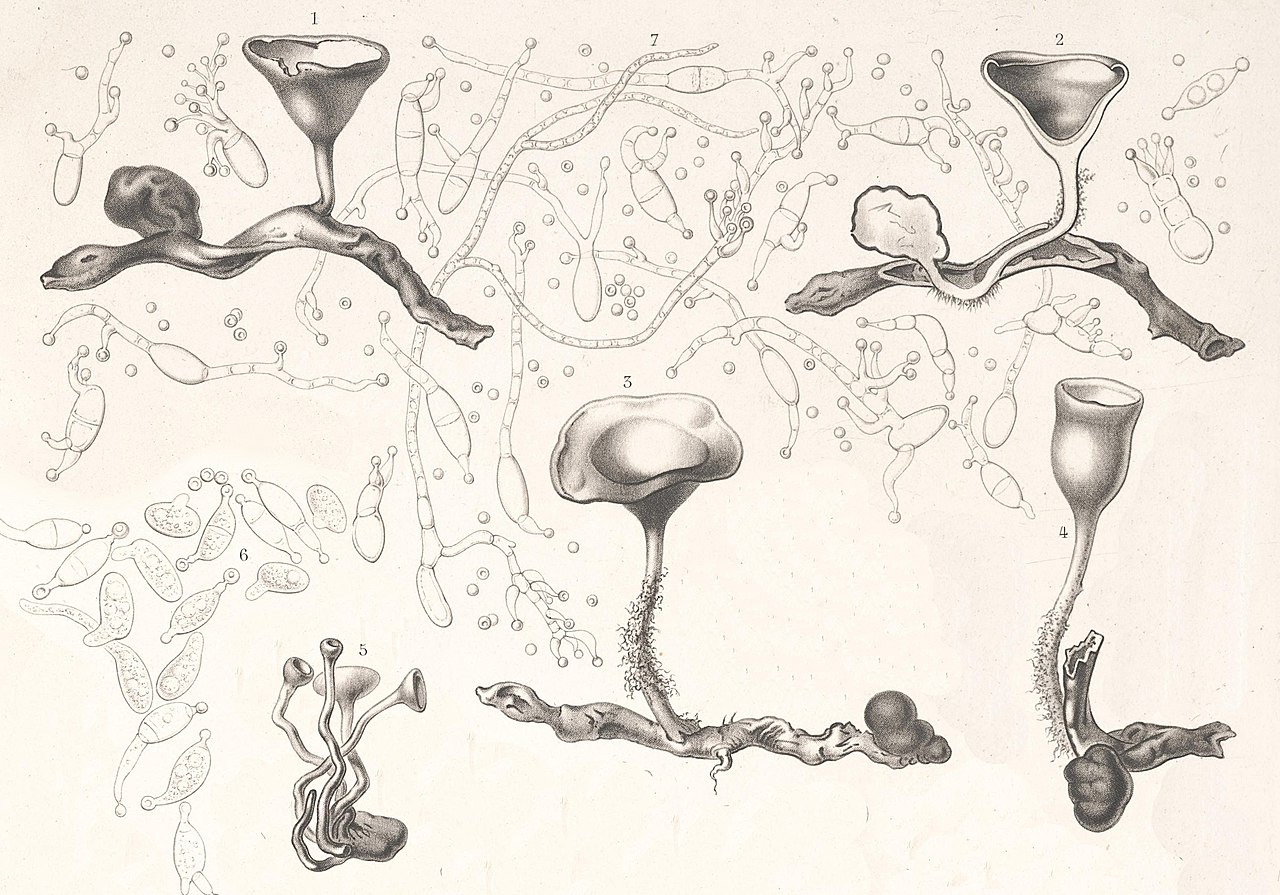
\includegraphics[width=0.9\textwidth]{Figures/PezizaTuberosa.jpg}
        \caption{Caption for figure 1.}
        \label{fig:figure-02.1}
    \end{subfigure}
    \hspace{.5cm} % Adjust the space as needed.
    \begin{subfigure}{0.45\textwidth}
        \centering
        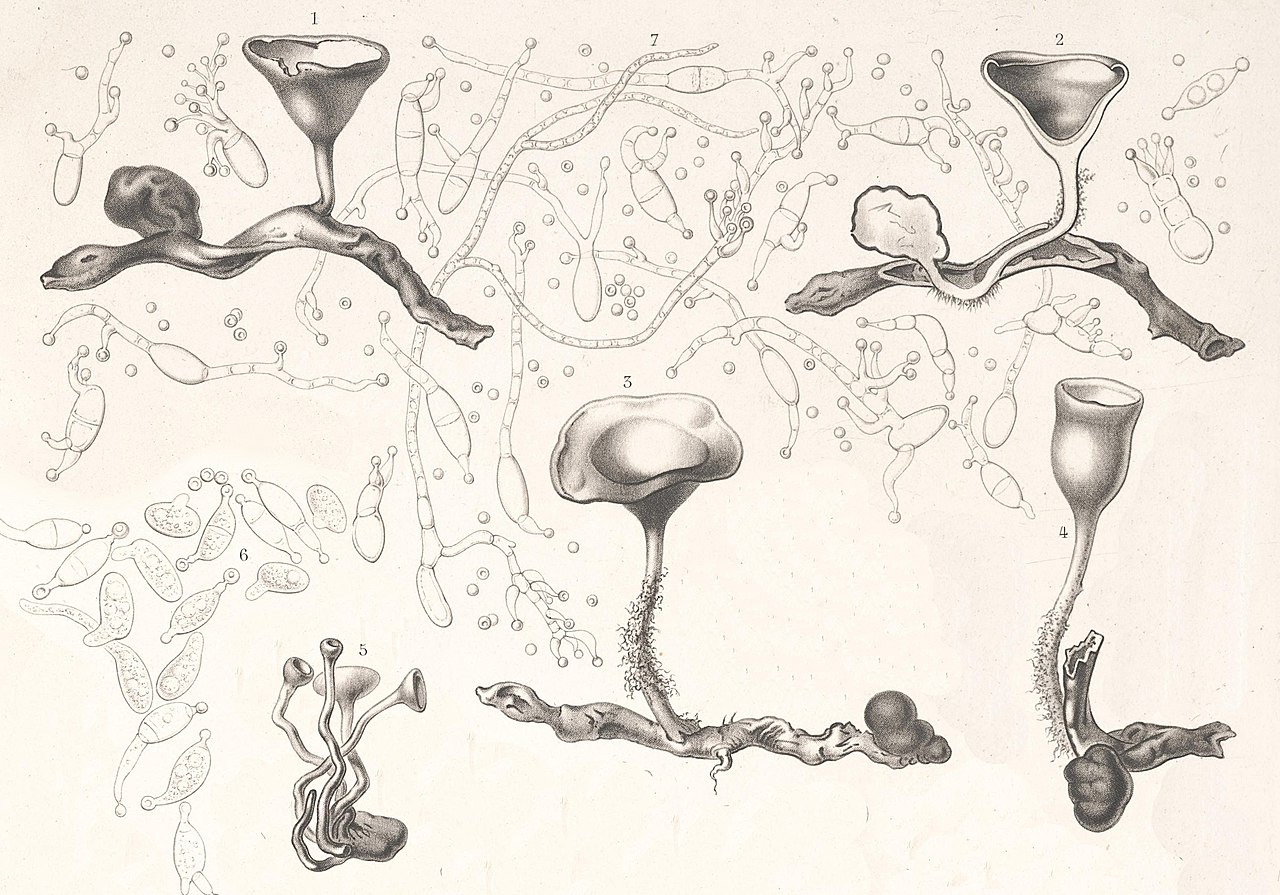
\includegraphics[width=0.9\textwidth]{Figures/PezizaTuberosa.jpg}
        \caption{Caption for figure 2.}
        \label{fig:figure-02.2}
    \end{subfigure}
    \caption{Overall caption of the figure.}
    \label{fig:figure-02}
\end{figure}

\section{Tables}
Tables are vital for presenting findings effectively. This chapter explores techniques for conveying information through tables using various template environments. Defining tables in \LaTeX\ seems complex, but this template simplifies the process.

\begin{block}[tip]
Different table environments must be within a \texttt{\textbackslash begin\{table\}} environment and use \texttt{[!htpb]} float options for better placement. \textbf{This advice should be taken into consideration when positioning figures as well}.
\end{block}

\subsection{Tabular Environment}
The conventional \verb|\begin{tabular}| environment enables you to create a simple yet elegant table. \autoref{tab:table-01} is generated using a centering environment for added emphasis. It also incorporates the \verb|booktab| configuration for a more sophisticated table style.

\begin{table}[!htpb]
    \caption{A table showcasing the usage of the tabular environment.}
    \label{tab:table-01}
    \centering
    \begin{tabular}{llc}
        \toprule
        \textbf{Header 01} & \textbf{Header 02} & \textbf{Header 03} \\ 
        \midrule
        Lorem Ipsum         & Pharetra Dolor    & $\checkmark$  \\
        Amet Consectetuer   & Curabitur Aliquet & -             \\
        Praesent Mauris     & Praesent Libero   & $\checkmark$  \\
        \bottomrule
    \end{tabular}
\end{table}

\subsection{Tabularx Environment}
Employ the \verb|\begin{tabularx}| package to construct a table featuring automatically expanding multi-columns. To achieve this automatic behaviour for multi-columns, you can use the following environment: \verb|\begin{tabularx}{\textwidth}{lX}|, where \verb|X| is the column that will function as a multi-column. Use \verb|C| to centre the multi-column, and \verb|L| and \verb|R| to align left and right respectively. \autoref{tab:table-02} showcases the usage of the \verb|\begin{tabularx}| environment.

\begin{table}[!htpb]
    \caption{A table showcasing the usage of the tabularx environment.}
    \label{tab:table-02}
    \begin{tabularx}{\textwidth}{lX}
        \toprule
        \textbf{Header 01} & \textbf{Header 02} \\ 
        \midrule
        Foo Bar Baz & Quisque cursus, metus vitae pharetra auctor, sem massa mattis sem, at interdum magna augue eget diam. \\
        Ipsum Dolor & Vestibulum ante ipsum primis in faucibus orci luctus et ultrices posuere cubilia Curae; Curabitur aliquet quam id dui. \\
        Dolor Sit & Phasellus condimentum elementum justo, quis interdum est sagittis ac. Vestibulum non arcu sit amet justo lobortis semper. \\
        Amet Consectetuer & Integer nec odio praesent libero sed cursus ante dapibus diam sed nisi vestibulum non arcu. \\
        % Consectetuer Adipiscing & Nulla quis sem at nibh elementum imperdiet. Duis sagittis ipsum. Praesent mauris. \\
        \bottomrule
    \end{tabularx}
\end{table}

\subsection{Longtable Environment}
At times, when dealing with exceptionally lengthy tables, it becomes necessary to split them across multiple pages. In \LaTeX, this can be achieved using the \verb|\begin{longtable}| environment. This environment is slightly more complex than others, as you need to define the header twice: once for the initial appearance of the table and again for when the table spans additional pages. This repeated header ensures the reader can correctly identify the columns on subsequent pages. Feel free to consult \autoref{tab:table-03} for a detailed demonstration of how the \verb|longtable| environment works.

\begin{longtable}[c]{llll}
\caption{A table showcasing the usage of the longtable environment.}
\label{tab:table-03} \\
\toprule
\textbf{Names} & \textbf{E-Mails} & \textbf{Job/Role} \\ \midrule
\endfirsthead
%
\multicolumn{4}{c}%
{{\textit{\bfseries Table \thetable\ continued from previous page.}}} \\
\toprule
\textbf{Names} & \textbf{E-Mails} & \textbf{Job/Role} \\ \midrule
\endhead
%
\bottomrule
\addlinespace[1mm]
\multicolumn{4}{r}%
{{\textit{Continued on the next page.}}} \\
\endfoot
\bottomrule
%
\endlastfoot
%
Alice Johnson & alice.johnson@email.com & Project Manager \\
Bob Thompson & bob.thompson@email.com & Data Analyst \\
Charlie Davis & charlie.davis@email.com & Marketing Specialist \\
David Miller & david.miller@email.com & QA Tester \\
Emily White & emily.white@email.com & Graphic Designer \\
Frank Martin & frank.martin@email.com & HR Coordinator \\
Grace Turner & grace.turner@email.com & Financial Analyst \\
Henry Lee & henry.lee@email.com & System Administrator \\
Ivy Carter & ivy.carter@email.com & Customer Support \\
Jack Wilson & jack.wilson@email.com & Frontend Developer \\
Jane Reed & jane.reed@email.com & UX Designer \\
Kevin Evans & kevin.evans@email.com & Product Manager \\
Linda Adams & linda.adams@email.com & Accountant \\
Mike Hill & mike.hill@email.com & Network Engineer \\
Nina Garcia & nina.garcia@email.com & Business Analyst \\
Oliver Smith & oliver.smith@email.com & Sales Representative \\
Pamela Turner & pamela.turner@email.com & Legal Counsel \\
Quincy Brown & quincy.brown@email.com & IT Consultant \\
Rachel Moore & rachel.moore@email.com & Content Writer \\
Samuel White & samuel.white@email.com & Research Scientist \\ 
Amy Harris & amy.harris@email.com & Digital Strategist \\
Brian Cook & brian.cook@email.com & Operations Manager \\
Catherine Ross & catherine.ross@email.com & Brand Manager \\
Daniel Green & daniel.green@email.com & Database Administrator \\
Emma Taylor & emma.taylor@email.com & Social Media Manager \\
Felix Carter & felix.carter@email.com & Compliance Officer \\
Gloria Scott & gloria.scott@email.com & Procurement Specialist \\
Harold Bennett & harold.bennett@email.com & DevOps Engineer \\
Isla Cooper & isla.cooper@email.com & User Researcher \\
James Black & james.black@email.com & Mobile App Developer \\
Katie Brown & katie.brown@email.com & UI Designer \\
Leo Perez & leo.perez@email.com & Scrum Master \\
Megan Clark & megan.clark@email.com & Event Coordinator \\
Nathan Ward & nathan.ward@email.com & Security Analyst \\
Olivia Harris & olivia.harris@email.com & Corporate Trainer \\
Paul King & paul.king@email.com & Territory Manager \\
Queen Foster & queen.foster@email.com & Paralegal \\
Rebecca Adams & rebecca.adams@email.com & Copy Editor \\
Steven Martin & steven.martin@email.com & Robotics Engineer \\
\end{longtable}

\subsection{Complex Tables}
Creating intricate tables in \LaTeX\ can be a somewhat challenging task. Therefore, we highly recommend using the \href{https://www.tablesgenerator.com/}{Table Generator}. With this tool, you can design your table with the desired style and then easily copy and paste it into your document. This approach simplifies the process and helps ensure the accurate representation of complex tables in your \LaTeX\ document. However, it's crucial to keep in mind that a table should be easily comprehensible for the reader and should not be overly complex. \textbf{The complexity of a table may impede understanding.} For example, \autoref{tab:table-04} presents a table with intricate details.

\begin{table}[!htpb]
    \caption{A table showcasing the usage of the complex tables.}
    \label{tab:table-04}
    \centering
    \begin{tabular}{lcc}
        \toprule
        \multirow{2}{*}{\textbf{Component}} & \multicolumn{2}{c}{\textbf{Specifications}} \\
        \cmidrule(lr){2-3}
        & \textbf{Characteristic} & \textbf{Supported} \\
        \midrule
        \multirow{4}{*}{CPU} & Core Count (e.g., 8 Cores) & $\checkmark$ \\
        & Clock Speed (e.g., 3.6 GHz) & $\checkmark$ \\
        & Hyper-Threading & $\checkmark$ \\
        & Integrated Graphics & - \\
        \midrule
        \multirow{4}{*}{GPU} & CUDA Cores (e.g., 5120) & $\checkmark$ \\
        & Base Clock (e.g., 1.5 GHz) & $\checkmark$ \\
        & Ray Tracing Support & $\checkmark$ \\
        & Multi-GPU Support (SLI/CrossFire) & - \\
        \midrule
        \multirow{4}{*}{Memory} & Type (e.g., DDR5, GDDR6) & $\checkmark$ \\
        & Capacity (e.g., 16 GB) & $\checkmark$ \\
        & Memory Bandwidth (e.g., 448 GB/s) & $\checkmark$ \\
        & ECC Support & - \\
        \midrule
        \multirow{3}{*}{Motherboard Features} & PCIe 5.0 Support & $\checkmark$ \\
        & Wi-Fi 6E & $\checkmark$ \\
        & Thunderbolt 4 & - \\
        \bottomrule
    \end{tabular}
\end{table}

\section{Lists}
Creating lists in \LaTeX\ is straightforward, offering various options to suit your needs. You can generate a bullet list using \verb|\begin{itemize}|, or opt for a numbered list with \verb|\begin{enumerate}|. Below is an example with the \verb|\begin{itemize}| environment.

\begin{itemize}
  \item List entries start with the \verb|\item| command.
  \item Individual entries are indicated with a black dot, a so-called bullet.
  \item The text in the entries may be of any length.
\end{itemize}

As mentioned earlier, you can generate a numbered list using the \verb|\begin{enumerate}| environment. Here is an example:

\begin{enumerate}
  \item Items are numbered automatically.
  \item The numbers start at 1 with each use of the \verb|enumerate| environment.
  \item Another entry in the list.
\end{enumerate}

You can also nest list entries by creating a list inside another list of the same type. Here is an example:

\begin{enumerate}
    \item First level item
    \item First level item
    \begin{enumerate}
        \item Second level item
        \item Second level item
    \begin{enumerate}
        \item Third level item
        \item Third level item
    \end{enumerate}
    \end{enumerate}
\end{enumerate}

\begin{block}[tip]
Please note that the labels change automatically regardless of the environment being the same for every list. \textbf{This demonstrates that there's no need to worry about changing the environment for something different.}
\end{block}

You can also modify the label of your list to something entirely different that suits your needs. To accomplish this, insert a new \verb|\item| and enclose your desired label in square brackets. For example, \verb|\item[!]| will result in an exclamation point as your new label. Below are some examples of modified labels.

\begin{itemize}
  \item This is my first point
  \item Another point I want to make 
  \item[!] A point to exclaim something!
  \item[$\blacksquare$] Make the point fair and square.
  \item[] A blank label?
\end{itemize}

Finally, you can create a description list. Unlike having a bullet point or a numbered label, a description list enables you to use custom descriptions that suit your list. In the example below, there are three \verb|\item| entries: one without a label, and two with descriptions.

\begin{description}
    \item[Item 1:] This is the first item with a description.
    \item[Item 2:] Another item with a different description.
    \item An item without a specific label.
\end{description}

\section{Code Listings}
At times, you may want to include source code from your programs and applications within your document. To achieve this, you can use two nested environments: \verb|\begin{listing}| to create a listing with both caption and label, and \verb|\begin{minted}| for code highlighting. \autoref{listing:c-code} provides an example of a source code in C.

\begin{listing}[!htpb]
\caption{Hello world in C.}
\label{listing:c-code}
\begin{minted}{c}
#include <stdio.h>
int main() {
   printf("Hello, World!"); /* printf() outputs the quoted string */
   return 0;
}
\end{minted}
\end{listing}

The code mentioned above was inserted into the document. However, an alternative approach is to input your code from an external file. To do so, you just need to use the command \verb|\inputminted{CODE_LANGUAGE}{FILE}|. Of course, you should place that command inside of the \verb|\begin{listing}| environment. \autoref{listing:haskell-code} illustrates an example of Haskell source code that has been input from an external file.

\begin{listing}[!htpb]
\caption{Factorial in Haskell.}
\label{listing:haskell-code}
\inputminted{haskell}{Code/Factorial.hs}
\end{listing}

In some cases, when you simply want to highlight a specific command, it's recommended not to use \verb|listing| or \verb|minted|. Instead, you should utilise the \verb|\verb| command for inline highlighting or the \verb|\begin{verbatim}| environment for longer sections of highlighted code. An example of a lengthy \verb|verbatim| section is provided below, demonstrating how to create a \verb|listing| with an input code:

\begin{verbatim}
\begin{listing}[!htpb]
    \inputminted{CODE_LANGUAGE}{FILE}
    \caption{TEXT}
    \label{TEXT}
\end{listing}
\end{verbatim}

Sometimes it is necessary to display longer code that occupies more than one page. For this purpose, please use the environment \verb|\begin{longlisting}|. This environment will easily break your code into multiple pages for better readability without you worrying about the size of your code. An example is shown below in \autoref{listing:lisp-code}.

\begin{longlisting}
\caption{A sample of functions in Lisp.}
\label{listing:lisp-code}
\begin{minted}{lisp}
(defun factorial (n)
  "Calculate the factorial of a number."
  (if (zerop n)
      (* n (factorial (1- n)))))

(defun fibonacci (n)
  "Calculate the nth Fibonacci number."
  (cond ((zerop n) 0)
        ((= n 1) 1)
        (t (+ (fibonacci (1- n)) (fibonacci (- n 2))))))

(defun gcd (a b)
  "Calculate the greatest common divisor of a and b."
  (if (zerop b)
      a
      (gcd b (mod a b))))

(defun primes-up-to (limit)
  "Return a list of all prime numbers up to LIMIT."
  (let ((primes '()))
    (loop for i from 2 to limit
          unless (some (lambda (p) (zerop (mod i p))) primes)
          do (push i primes))
    (nreverse primes)))

(defun example-function (x)
  "An example function to demonstrate Lisp capabilities."
  (let ((result (list (factorial x)
                      (fibonacci x)
                      (gcd x 10)
                      (primes-up-to x))))
    (format t "Factorial of ~A: ~A~%" x (factorial x))
    (format t "Fibonacci of ~A: ~A~%" x (fibonacci x))
    (format t "GCD of ~A and 10: ~A~%" x (gcd x 10))
    (format t "Primes up to ~A: ~A~%" x (primes-up-to x))
    result))

(example-function 10)
\end{minted}
\end{longlisting}

\section{Equations}
When writing equations and other mathematical expressions, \LaTeX~is a powerful and versatile tool. You can enter a formula in inline mode using the environment \verb|\(FORMULA\)| or use \verb|\begin{equation}| to display it in ``math mode'' with numbering. If you prefer not to display the equation number, you can use the environment \verb|\[FORMULA\]|.

\vspace{.875em}
\textbf{Example:} In physics, the mass-energy equivalence is expressed by the equation \(E=mc^2\), discovered in 1905 by Albert Einstein. In natural units ($c = 1$), the formula (\ref{eq:equation-01}) expresses the identity:

\begin{equation}
\label{eq:equation-01}
E=m
\end{equation}

\textbf{Example:} Below is a equation -- \textit{without numbering} -- for the regularised loss function in supervised learning, combining the average prediction loss over the training dataset and an $L_2$ regularisation term to prevent overfitting:

\[
\mathcal{L}(\boldsymbol{\theta}) = \frac{1}{N} \sum_{i=1}^{N} \ell(y_i, f(\mathbf{x}_i; \boldsymbol{\theta})) + \lambda \|\boldsymbol{\theta}\|_2^2
\]

Equations can be a bit challenging to create, so we advise using an online editor, like the \href{https://latexeditor.lagrida.com/}{LaTeX Equation Editor}. Simply build your formulas there and copy and paste them into your document, either inline or in a math block, as shown above.

\section{Footnotes}
Sometimes it is important to present information that is not central to the main text in a footnote. In \LaTeX\, this can be easily achieved using the command \verb|\footnote{TEXT}|. The text will appear at the bottom of the page\footnote{This is a simple footnote.}.

If you want to use footnotes within tables, it is best to reconsider, as \LaTeX\ does not provide an easy way to handle them. Instead, you can place a ``*'' wherever you want the footnote reference to appear. Then, below the table \textbf{but before ending the table environment}, place the ``*'' along with the footnote text. This will create a similar footnote, but it will appear below the table rather than at the bottom of the page.

%%% Bibliography %%%
\renewcommand{\refname}{Bibliography}
\printbibliography[title={\refname},heading=bibintoc]

%%% Appendices: Work that *YOU* Developed %%%
% \appendix
% \ifthenelse{\equal{\LanguageOption}{portuguese}}{
    \addtocontents{toc}{\protect\contentsline{chapter}{Apêndices}{}{}}
}{
    \addtocontents{toc}{\protect\contentsline{chapter}{Appendices}{}{}}
}

\ifthenelse{\equal{\MediaOption}{paper}}{\blankpage}{\clearpage}
\begin{center}
    \crimsonfont
    \thispagestyle{empty}
        
    \vspace*{\fill}
    \ifthenelse{\equal{\LanguageOption}{portuguese}}{%
        {\LARGE\fontsize{26}{26}\selectfont\textcolor{maincolor}{Apêndices}\par}
    }{%
        {\LARGE\fontsize{26}{26}\selectfont\textcolor{maincolor}{Appendices}\par}
    }
    \vspace*{\fill}
\end{center}
\MediaOptionLogicBlank
% \chapter{Showcasing the First Appendix}
\guideinfo{Appendices contain supplementary material \textbf{created by the author} that enhances the reader’s understanding of the dissertation while not being essential for following the primary narrative. These sections often include detailed tables, figures, complex calculations, or materials like survey questions and interview transcripts produced in the course of the research. The appendices allow readers to explore the research in greater detail, offering a deeper insight into methods and findings without interrupting the main body of work.}
% % Recommended dimensions for a landscape layout; adjust as needed.
\begin{landscapemode}{297mm}{420mm}
    \chapter{Showcasing the Second Appendix}
    \blindtext[5]
\end{landscapemode}

% %%% Annexes: Work that *YOU DID NOT* Develop %%%
% \ifthenelse{\equal{\LanguageOption}{portuguese}}{
    \addtocontents{toc}{\protect\contentsline{chapter}{Anexos}{}{}}
}{
    \addtocontents{toc}{\protect\contentsline{chapter}{Annexes}{}{}}
}

\setcounter{chapter}{11} % To start at the "L" chapter.
\MediaOptionLogicAnnexes
\begin{center}
    \crimsonfont
    \thispagestyle{empty}
        
    \vspace*{\fill}
    \ifthenelse{\equal{\LanguageOption}{portuguese}}{%
        {\LARGE\fontsize{26}{26}\selectfont\textcolor{maincolor}{Anexos}\par}
    }{%
        {\LARGE\fontsize{26}{26}\selectfont\textcolor{maincolor}{Annexes}\par}
    }
    \vspace*{\fill}
\end{center}
\MediaOptionLogicBlank
% \chapter{Showcasing the First Annex}
\guideinfo{Annexes are supplementary sections in a dissertation that provide additional information or external documents not essential to the main arguments but that support or complement the research. Unlike appendices, \textbf{annexes generally contain material that was not developed by the author}, such as reports, legal documents, or published datasets from external sources. This information is placed separately to keep the main content concise, allowing readers access to relevant external references without disrupting the dissertation's flow.}

%%% Back Page %%%
\ifthenelse{\equal{\MediaOption}{paper}}{\blankpage}{}

\clearpage
\null
\thispagestyle{empty}

\ifthenelse{\equal{\CoverOption}{classic}}{
    \newcommand\BackgroundPicBackPage{%
    \put(0,0){%
    \parbox[b][\paperheight]{\paperwidth}{%
    \vfill
    \centering
    
\includegraphics[width=\paperwidth,height=\paperheight,keepaspectratio]{Figures/Theme/Back-Page-Blue.pdf}%
    \vfill
    }}}
}{
    \newcommand\BackgroundPicBackPage{%
    \put(0,0){%
    \parbox[b][\paperheight]{\paperwidth}{%
    \vfill
    \centering
    
\includegraphics[width=\paperwidth,height=\paperheight,keepaspectratio]{Figures/Theme/Back-Page-BG-W.pdf}%
    \vfill
    }}}
}

\AddToShipoutPictureBG*{\BackgroundPicBackPage}

\newgeometry{margin=1.98cm, top=1.47cm, bottom=1.47cm}
\noindent\clearpage
\restoregeometry

\end{document}